\documentclass[a4paper,11pt]{kth-mag}
\usepackage[T1]{fontenc}
\usepackage{textcomp}
\usepackage{lmodern}
\usepackage{graphicx}
\usepackage[utf8]{inputenc}
\usepackage[swedish,english]{babel}
\usepackage{modifications}

% http://library.uwl.ac.uk/find/guides/general/harvard_reference.html

\title{Title}
\subtitle{Subtitle}
\foreigntitle{Titel på svenska}
\author{Björn Tegelund\\Johan Wikström}
\date{November 2003}
\blurb{Bachelor's Thesis at CSC\\Supervisor: Petter Ögren\\Examiner: Mårten Björkman}
\trita{TRITA xxx yyyy-nn}
\begin{document}
\frontmatter
\pagestyle{empty}
\removepagenumbers
\maketitle
\selectlanguage{english}
\begin{abstract}
  This is a skeleton for KTH theses. More documentation
  regarding the KTH thesis class file can be found in
  the package documentation.

\end{abstract}
\clearpage
\begin{foreignabstract}{swedish}
  Denna fil gfwfqwfwqfqer ett avhandlingsskelett.
  Mer information om \LaTeX-mallen finns i
  dokumentationen till paketet.

\end{foreignabstract}
\clearpage
\tableofcontents*
\mainmatter
\pagestyle{newchap}
\chapter{Introduction}

\section{Background}

Genetic algorithms are algorithms that emulate evolution to achieve a optimal solution to a problem\footnote[1]{Proof}. 
These algorithms have many uses and we wanted to investigate whether the phenomena which occur in nature
due to evolution also occurs when using genetic algorithms. In nature evolution has spawned a wide variety
of survival strategies such as adaptation, camouflage colours and mimicry. Genetic algorithms however, are 
very simplified mathematical models of these mechanisms which means that these phenomena might not occur 
at all.

\section{Scope and Objectives}

Main objective:\\
Compare RBF-based and "linear" brains.\\
By: Forcing them to adapt certain genetic phenomena such as adaptation (learning), co-evolution and extinction, mimicry, group forming and co-operation prioritised in the order presented (as increasingly complex behaviour and difficulty to simulate).\\

Questions:\\
How quickly do they learn?\\
Can both kinds of brains do the same things?\\
Pros and cons for each brain architecture\\
RBF-based predators vs linear prey, vice versa.\\

Evolution of brains using RBF functions and evolutionary algorithms.

\section{Achievements}

\chapter{Technical Overview}

\section{Genetic Algorithms}

\subsection{Overview}
What are genetic algorithms?\\
How are they typically used?\\
How do they relate to genetics and evolution?\\
Overview of algorithm\\

\subsection{Selection}
\subsection{Fitness}
\subsection{Mutation}
\subsection{Crossover}

\section{Radial Basis Functions}
\subsection{Overview}

\begin{figure}
\centering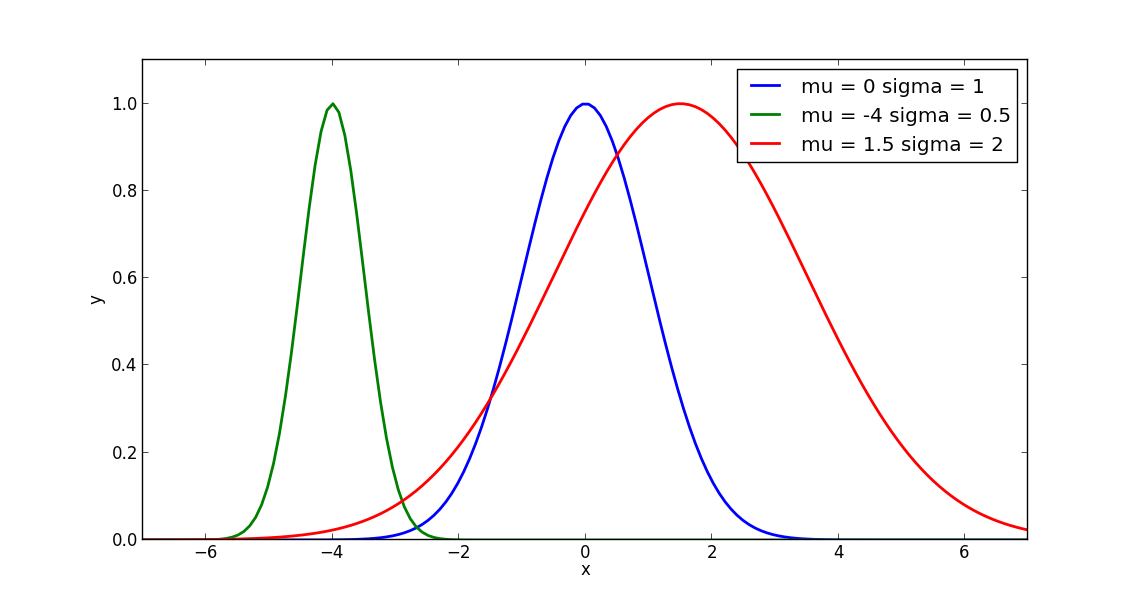
\includegraphics[scale=0.5]{rbf_1d.png}
\caption{Three one-dimensional RBFs with varying $\mu$ and $\sigma$ values.}
\end{figure}

A radial basis function (RBF) is a bell-shaped function which value depends on the distance from some origin, denoted $\mu$ in the formula.  Radial basis functions are commonly used in neural networks as a way to encode input information. They are favourable to use as they have locality, something which linear functions do not. In particular they are used for function approximation, as any function can be approximated as the sum of a number of weighted radial basis functions. A property of radial basis functions which can both be interpreted as an advantage and disadvantage is that their value never exceeds 1, compared to a linear function which can grow to infinitely high or low numbers.

Radial basis functions are commonly implemented using a formula such as \ref{RBF_1}, which is a three-dimensional function centred around $(\mu _{x}$, $\mu _{y}$, $\mu _{z})$. The width of the bell-curve in each dimension is determined by $\sigma _{x}$, $\sigma _{y}$ and $\sigma _{z}$ respectively.

\begin{figure}
\begin{equation}
f(x,y,z) = \exp(-(\frac{(x-\mu_{x})^{2}}{2 \sigma _{x}^{2}} + \frac{(y-\mu_{y})^{2}}{2 \sigma _{y}^{2}} + \frac{(z-\mu_{z})^{2}}{2 \sigma _{z}^{2}}))
\end{equation}
\caption{A three-dimensional radial basis function.\label{RBF_1}}
\end{figure}

\chapter{Implementation}
\section{Model}
\subsection{Simulation in Python}
Square world with walls, circular inhabitants with antennae\\
Good and bad food sources\\
Predators?\\
Possible modifications to enforce different behaviour?\\
What libraries will we use? Why?\\
Optimisations?\\

\subsection{Methods of Enforcing Behaviour}
Adding input\\
Additional terms in brain calculations\\
Adding predators\\
More kinds of food\\
Being able to see more things in the world\\
Placing objects into the world\\

\subsection{RBF-Based Decision Making}

When input is received by a creature, it is in form of eight numbers, four for each antenna. Three of the inputs for each antenna are the red-, green- and blue components of the currently detected object's colour. The fourth input is zero when no object is detected and one when an object is. The three colour-based inputs are then used in several three-dimensional radial basis functions. For each antenna a $\Delta r$ (change in rotation) and $\Delta s$ (change in speed) is computed by summing the function values and normalising them. The $\Delta r$ and $\Delta s$ for each antenna are then grouped and used by the creature to change it's rotation and speed. See equation \ref{RBF_decide}.

\begin{figure}
\begin{equation}
\Delta s _{left} = f(\mathbf{x} _{left})
\end{equation}
\caption{Calculating the $\Delta s$ for the left eye, using the input vector $\mathbf{x} _{left}$ corresponding to the colours of the object detected using the left antenna.\label{RBF_decide}}
\end{figure}

Each radial basis function also has a $\sigma$ and $\mu$ which are decided by the creature's genes. $\sigma$ and $\mu$ are in the ranges of $[0,1]$ and $[-1,1]$ respectively. In practice this means that the creatures' change in speed and rotation, when detecting an object in each antenna, depend on their genetic makeup.

The difference between using radial basis functions and linear functions is that you have a much larger possibility to approximate any decision-making strategy. For example an RBF-based brain could make the distinction between different shades of green and thus react differently to them, while a linear function could only decide if more green is better or worse.

\subsection{Genetic Algorithm}
What kind of genetic algorithm do we plan to use?\\
Fitness, crossover, mutation, selection, which ones?\\
Flow chart of our algorithm\\
NSGA-II\\

\subsection{Experiments}
(In every experiment linear and RBF are compared, eventually mixed)\\
Interested in:\\
Time to maximal fitness\\
Highest possible fitness\\
\begin{itemize}
\item Adaptation 1. Finding and eating food
\item Adaptation 2. Finding and eating food, avoiding "bad" food
\item Co-evolution and extinction 1. Predator vs prey, prey eats food as in first experiment. (bushes are bad for predators)
\item Speciation and co-operation 1. Allow the creatures to evolve which "colour" food they can eat, attempt to create two separate species from one, one species eating green bushes and one red.
\item Mimicry 1. Making the prey mimic bushes or predators to avoid being eaten.
\item Mimicry 2. Predators attempt to mimic bushes to make prey run into them.
\item Group forming 1. Rerun all previous experiments, but with the ability to detect the nearest creature of the same species.
\end{itemize}


\chapter{Results}
\section{Simulation results}
\subsection{Observed Behaviours}
\section{Discussion}
\subsection{Constraints and problems}
Performance problems\\
Other unexpected problems?\\

\section{Conclusions and Future Work}

\chapter*{References}
\begin{enumerate}
\item Montana, D. J.,  and Davis, L. (1989, August). Training feedforward neural networks using genetic algorithms. In \emph{Proceedings of the eleventh international joint conference on artificial Intelligence} (Vol. 1, pp. 762-767).
\item Langton, C. G., and Shimohara, T. (Eds.). (1997). \emph{Artificial Life V: Proceedings of the Fifth International Workshop on the Synthesis and Simulation of Living Systems} (Vol. 5). Mit Press.
\end{enumerate}

\appendix
\addappheadtotoc
\chapter{RDF}\label{appA}

\begin{figure}[ht]
\begin{center}
And here is a figure
\caption{\small{Several statements describing the same resource.}}\label{RDF_4}
\end{center}
\end{figure}

that we refer to here: \ref{RDF_4}
\end{document}
